\documentclass{report}
\usepackage{blindtext}
\usepackage[utf8]{inputenc}
\usepackage{hyperref}
\usepackage{amsmath}
\usepackage{graphicx}
\usepackage[export]{adjustbox}
\usepackage{float}

\begin{document}

\title{ - project report}
\begin{titlepage}
	\centering
	{\scshape\LARGE FMFI UK \par}
	\vspace{1cm}
	{\scshape\Large Project report\par}
	\vspace{1.5cm}
	{\huge\bfseries Victory prediction for World of Tanks\par}
	\vspace{2cm}
	{\Large\itshape Matúš Zeleňák\par}


	\vfill

% Bottom of the page
	{\large \today\par}
\end{titlepage}

\section{Abstract}

Assessing the strength of teams is a common struggle of every player participating in a competitive online video game, as is the popular FPS tank shooter World of Tanks. By having a solid grasp of every teams strong and weak elements, one can accordingly adjust his own playstyle in order to defeat the enemy. Detailed analysis might consist of considering the strength of every single player, but human mind isn't particularly good at drawing conclusions from a large amount of variables and dependencies. Having a single number describing the predicted chance to win (or just the most probable outcome) is simpler to process.

In this work we aim to apply the classification power of neural networks in order to predict a game outcome based on the initial state of the game. 

\section{Problem definition}

World of Tanks (WoT) is multiplayer game where two teams stand against each other 
on a battlefield map commanding their tank of choice. In each of the possible game modes the victorious team is determined either by eliminating all of the enemy vehicles, or by capturing/defending the enemy/friendly base. Destroyed vehicles do not respawn.

Despite some RNG elements, the game is heavily skill based, rewarding good positioning, map awareness, aiming skills, timing, target prioritization and many others. Due to these factors, there are significant skill gaps between players (worst having 40\% or worse global winrate, the best having over 65\%). 

Player skill however only takes one as far, as the tank capabilities allow. The game currently has vehicle research trees with 10 levels (tiers). Tank of each subsequent tier generally becomes stronger in the qualities of its class, of which there are:

\begin{enumerate}
	\item{Heavy tank - great armor, good guns, poor mobility}
	\item{Medium tank - medium armor, good guns, good mobility}
	\item{Tank Destroyer - medium armor, great guns, medium mobility, good camouflage}
	\item{Light Tank - poor armor, poor guns, great mobility and camouflage}
	\item{Artillery - poor armor, indirect fire, poor mobility}
\end{enumerate}

From the above list, one can already see that there's a rock-paper-scissors mechanic in place, where heavy tanks counter mediums, mediums counter lights, lights counter artillery, which counters heavy tanks...

Teams for each battle are assembled by the game server which draws players (in their tanks) from the queue and attempts to construct a balanced match-up.

It does so by using a mirror template system - this means that if one team has a tank of certain class and tier, the other team receives a tank of the same tier and class as well.

What the matchmaker does \emph{not} take into account is player skill. This can lead to unbalanced games, especially in the edge cases where the top-tier players on one team are significantly better than the ones on the other. 

To make matters worse (balance-wise), there are more contributing factors. One of such is the fact, that not all tanks of the same tier and class are equally powerful. Moreover, since the maps are not symetrical and teams spawn in clusters on the opposite sides, the spawn point also influences the team balance. Furthermore, the strenghts of certain tank can be greatly accentuated or diminished by the chosen map. Both of these are issues with the game balance which are always a subject to change.

When loading into the battle, there's no way for a player to see the skill characteristics of other players without the use of game modifications. There are 3rd party sites and APIs where such data can be obtained (as do the mentioned mods). An example can be seen here (my personal characteristics) 
\url{https://wot-life.com/eu/player/Whiskas_GJH}

Apart from the straight-forward statistics like winrate and average damage dealt, there is also one metric that stirs the most controversy in the community - WN8 rating. This number is supposed to represent the overall performance of the player. A side objective of our work is to determine, how telling this metric is compared to the others.

\section{Inputs and dataset creation}

World of Tanks has an option of saving a replay after each game - a file that contains all of the visible actions of both teams and makes it possible to rewatch the battle to the finest detail.

This file thus contains the information necessary for our project:
\begin{enumerate}
	\item{Teamlists describing the tanks in both teams}
	\item{The map and spawn location of both teams}
	\item{Results - victory/loss/draw, performance for each player}
\end{enumerate}

We obtained majority of our replays from our own gameplay over the last month (around 1170 instances) 
Additionally, we asked people on various media (Reddit, WoT forum, WoT ingame friendlist) to send in 
their own games, of which we received 961. In total we thus collected around 2130 replays.

\subsection{Data processing}

The replay file format is a binary proprietary type. Fortunately, there exists a person who maintains an up-to-date software capable of mass-converting these replays into JSON files. 
\url{http://forum.worldoftanks.eu/index.php?/topic/185348-0921-wot-replay-analyzer-wip-2-27122017/}


These raw JSON files however contain too much information and in a messy structure. Next we run a script that does the following:
\begin{enumerate}
	\item{Discards incomplete replays}
	\item{Strips the JSON file of unneccessary information}
	\item{Makes a query for statistics for each player}
\end{enumerate}

For the second part of above section we use the site \url{wot-life.com} .For a pair (player, tank) we 
save the following information
\begin{enumerate}
	\item{ General statistics
		\begin{enumerate}
			\item Winrate
			\item Battles played
			\item WN8
		\end{enumerate}
	}
	\item{ Tank statistics
		\begin{enumerate}
			\item Winrate
			\item Battles played
			\item WN8
			\item Average damage
		\end{enumerate}
	}
	\item{ Tank information
		\begin{enumerate}
			\item Name
			\item Tier
			\item Class
		\end{enumerate}
	}
\end{enumerate}

Apart from teamlists, we also save the name of the map, spawn points for both teams and the game outcome. If for any reason we couldn't obtain data for even a single player, we discarded the whole replay as to not introduce errors.

Another step is to obtain the statistics for particular maps and tanks. We used this website 
\url{http://www.vbaddict.net/wot.php}. 
We run a script that scrapes the global winrate for each of over 500 tanks, as well as winrates for both spawns on all 40 maps for all game modes. 
We store the results in separate JSON files.

\subsection{Difficulties with replay processing}

The most prominent problem arose from the fact that not all player statistics were accessible. 
We suspect this happens for three reasons:
\begin{enumerate}
	\item{Players in replays are identified by their nicknames, which they can change. Our queries therefore sometimes hit upon names which are no longer valid. Luckily for us, changing nicknames in this game costs money, so hardly anyone cares}
	\item{Recently, the developers of WoT enabled players to hide their statistics from public. Luckily, hardly anyone cares.}
	\item{Statistic tracking websites lag behind the actual game by a few hours. If a player in our replay just unlocked a new tank and we process the replay shortly after, this tank will not be found in the website's records}
\end{enumerate}

Because of aforementioned issues we were forced to ditch over 600 files, ending up with 1446 usable instances.

\section{State of the art methods today}

The only real attempt at predicting the game outcome has been made by the XVM community at
 \url{https://modxvm.com/} and incorporated in their modpack for the game. Apart from showing the 
player statistics in the teamlist, this mod was capable of making a win chance prediction.
The formula used for chance calculation is described in detail here:
\url{http://forum.wotlabs.net/index.php?/topic/15131-xvm-win-chance-prediction-algorithm/}

After several years of controversy the win prediction was removed as it encouraged toxic gameplay.

In our opinion, the XVM formula itself is rather controversial. The authors went to great lengths to count in 
objectively small factors like average tier played, or how much one player "sealclubbs", but completely 
overlooked decisive factors like already mentioned map spawns or specific vehicle winrate. 

Understandably there are not any formal papers studying how well the XVM works, several player however have devoted their time to their analyses:
\url{http://forum.worldoftanks.com/index.php?/topic/522269-how-accurate-are-xvm-predictions/}
\url{http://forum.worldoftanks.eu/index.php?/topic/468409-a-1000-battle-study-on-xvm-win-chance-accuracy/}

The bottom line is that the XVM is quite accurate for fairly unbalanced matches, but struggles to correctly predict 
result for close games. 

\section{Implementation details and obstacles}

We implemented the entire project in Python 3 using Keras as the neural network API.
Our pipeline is separated into several scripts:

\begin{enumerate}
	\item{
		process\_raw\_json.py - Script loads the JSON files produced by WoT Replay analyzer and performs the following for every file:
		\begin{enumerate}
			\item{Extracts the necessary information}
			\item{For every player obtains his statistics}
			\item{Merges the information into a new, simpler JSON file}
		\end{enumerate}
		}
	\item{
		scrape\_vbaddict.py - Script obtains the global winrates for every tank in the game as well as global spawn winrates for every map and saves to JSON
	}
	\item{
		construct\_dataset.py - Processes the simplified JSON replays into a data matrix and corresponding labels.
	}
	\item{
		heuristic.py - Here we tried to come up with alternate ways of predicting the outcome by methods simpler than machine learning as a benchmark.
	}
	\item{
		XVM.py - Truthfully recreated XVM winchance prediction as described in the abovementioned link.
	}
	\item{
		train\_model.py - This is where the actual neural network training happens, along with testing accuracy evaluation.
	}
	\item{
		visualize\_data.py - Result visualization
	}
\end{enumerate}

\subsection{Data matrix}

Let's take a better look at how we represent the data for the neural network.

First, we would like to make it apparent, that there are certain dependencies 
based on the vehicle tiers and classes. We therefore construct a $3 \times 5$ matrix for each team (let's call them $M^A, M^B$ ), 
where rows represent the tier spread in the battle and columns represent classes.

\[
M^X = 
\begin{bmatrix}
    x_{1,1} & x_{1,2}  & \dots  & x_{1,5} \\ \\
    \vdots & \vdots  & \ddots & \vdots \\
    x_{3,1} & x_{3,2}  & \dots  & x_{3,5}
\end{bmatrix}
\]

The cells of the matrix are initialized to vector of zeroes with length equal to the number of player parameters we take into account.

Afterwards we assemble for each player in team $X$ a vector of his (or his tank) qualities (in our case we picked the global tank winrate, player's winrate in said tank and his overall winrate).

\[ x_{tier, class} = 
\begin{bmatrix}
	wr_{tank}, & wr_{player}, & wr_{player,tank}
\end{bmatrix}
\]

We perform addition with this vector into the matrix $M^X$ according to the tier and class of the players tank.

$$M^X_{tier, class} = M^X_{tier, class} + x_{tier, class}$$

We perform the same action for the other team and their matrix.
In the end, we perform $M^A - M^B$, effectively creating a matrix containing a skill/quality difference between the teams for each tier and class.

A final touch includes flattening the difference matrix into a vector and appending the disparity in team's spawn winrates.
The end result is one row of data corresponding to one replay.

In order to ensure that our model learns to recognise symetrical cases, we create another row where instead of $M^A - M^B$ we do $M^B - M^A$. This also has the added benefit of having the same amount of positive/negative samples.

For each such row we also save a single integer $w \in \{0, 1\}$ noting which team won as well as a label describing the original filename for later outlier processing.

\section{Experimental evaluation and comparation}

In total, our dataset contains 2878 rows.
First, we shuffle the rows and separate $30\%$ of them as a testing set.
Next, we feed the remainding $70\%$ to the model.
We constructed 5 neural networks with 4 Dense layers. We train each of these nets on different four fifths of the set, using the remaining fifth as a validation set (leave-one-out method).

We observed that the networks don't suffer from overfitting, as the validation accuracy of each network stayed relatively close to the training accuracy (within $2\%$ range).

Next we computed predictions on the testing set from each network, and averaged the output classification confidencies. We then evaluated the predictions by marking those 
that had the confidence with over 50\% on the correct outcome as correct.

This way, we obtained on average 75\% prediction accuracy on test data. 

\subsection{Heuristic method}

Our heuristic method computes a team strength by summing up the product of the same parameters we used for our data matrix

$$S_{team} = \sum_{player \in team}{s_{player}} \times spawn\_advantage$$
$$s_{player} = wr_{tank} \times wr_{player} \times wr_{tank,player}$$

We then compare $S_{team}$ for both teams and proclaim the stronger team as victorious.

This method yielded 71\% prediction accuracy. The more elaborate we made the formula (accounting for tiers, classes, map types etc) the less accurate the formula became.

\subsection{Comparison with XVM}

On the same set of inputs as was the testing set for our model we also ran XVM prediction.
This yielded only a 0.69\% prediction in win accuracy. However, we took a deeper look at the data and visualized some of the comparisons in the following figures.

In the figure \ref{fig:chance} we can see how the confidence in an outcome (or win chance) correlate with the actual win percentage of the games. Since XVM doesn't predict the extreme cases as often, we were forced to drop the few samples ($< 5$) it found on the edges as to not skew the results. 
Our model seems to perform similarly, if not a bit better than the XVM. Since the relation between our model's confidence and actual win percentage is near linear, we will treat the confidence as the predicted win chance from now on.

\begin{figure}[H]
\hspace{-80pt}
  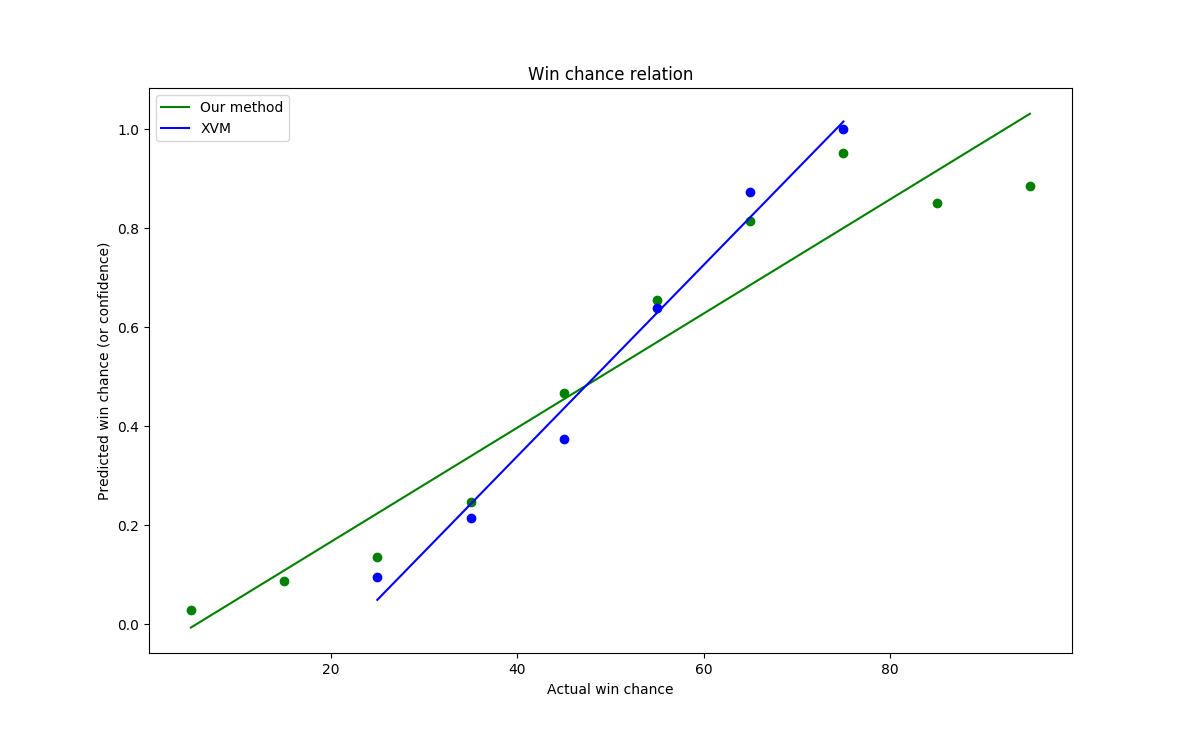
\includegraphics[width=500px]{confidence_to_chance.png}
  \label{fig:chance}
\end{figure}

In the figure \ref{fig:confidence} we can observe the relation between the models increasing win chance in a particular outcome and the accuracy it achieves with the win chance above certain treshold.
We can see that the XVM model gains accuracy faster with the increasing win chance, which makes it superior to our model.

\begin{figure}[H]
\hspace{-80pt}
  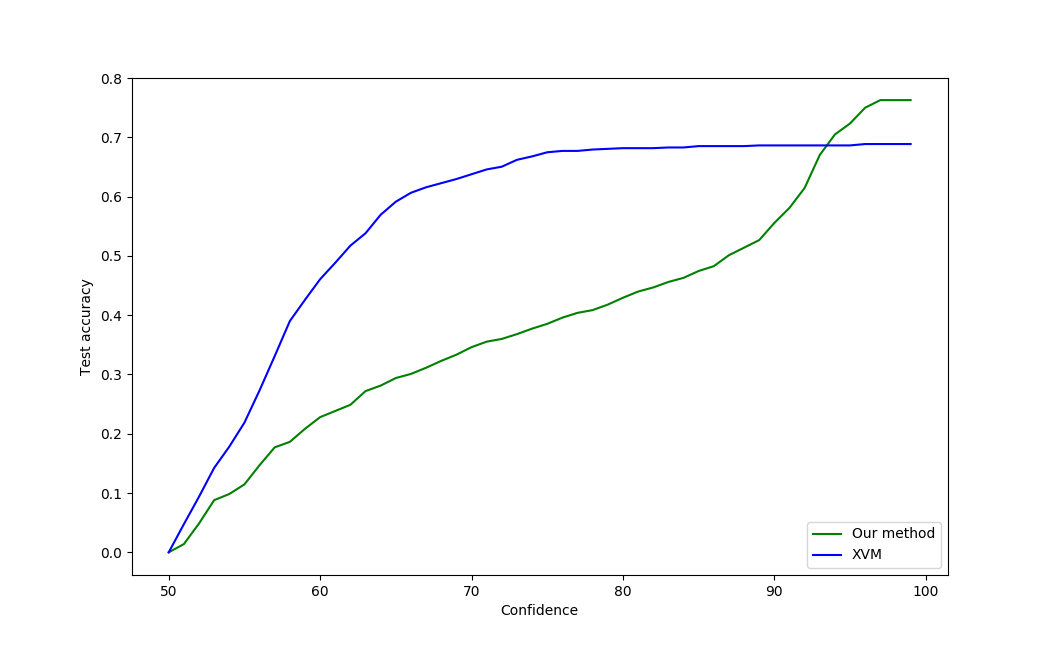
\includegraphics[width=500px]{confidence_to_accuracy.png}
  \label{fig:confidence}
\end{figure}

Subsequent figure \ref{fig:distribution} we plot the distribution of win chances across all the games.
The results here a bit undermine our assumption that the confidence is a good substitute for win chance, as it would mean that the matchmaker is rigged and produces heavily unbalanced games more often than it should under assumption it really picks players randomly. XVM models the distribution closer to the gaussian, as should be in the ideal case.

\begin{figure}[H]
\hspace{-80pt}
  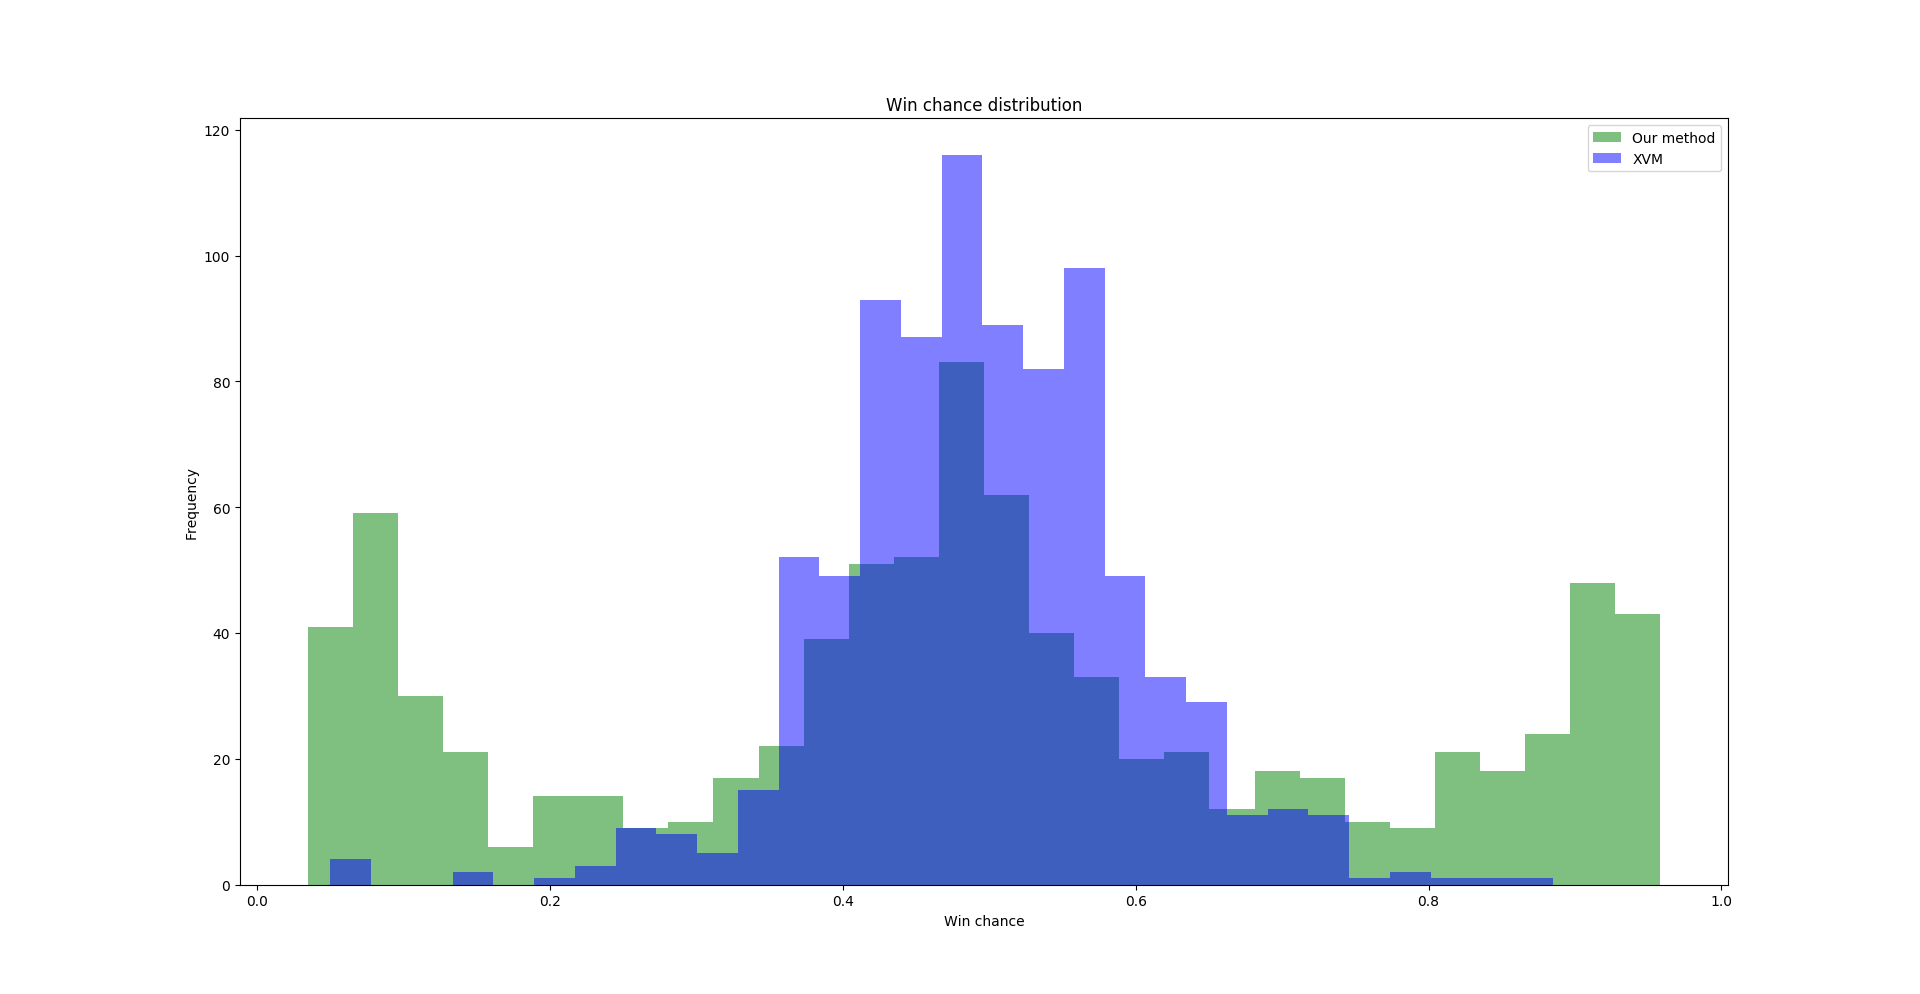
\includegraphics[width=500px]{winchance_distribution.png}
  \label{fig:distribution}
\end{figure}

The final figure depicts the distribution of missclasified examples with relation to the predicted win chances disparity (50\% win chance has disparity 0, 75\% has 50 and so on). As can be expected, most of the missclassified examples happen when the win chance is close to 50\%. Again, XVM performs better as it has very few outliers in the high win chance area.

\begin{figure}[H]
\hspace{-80pt}
  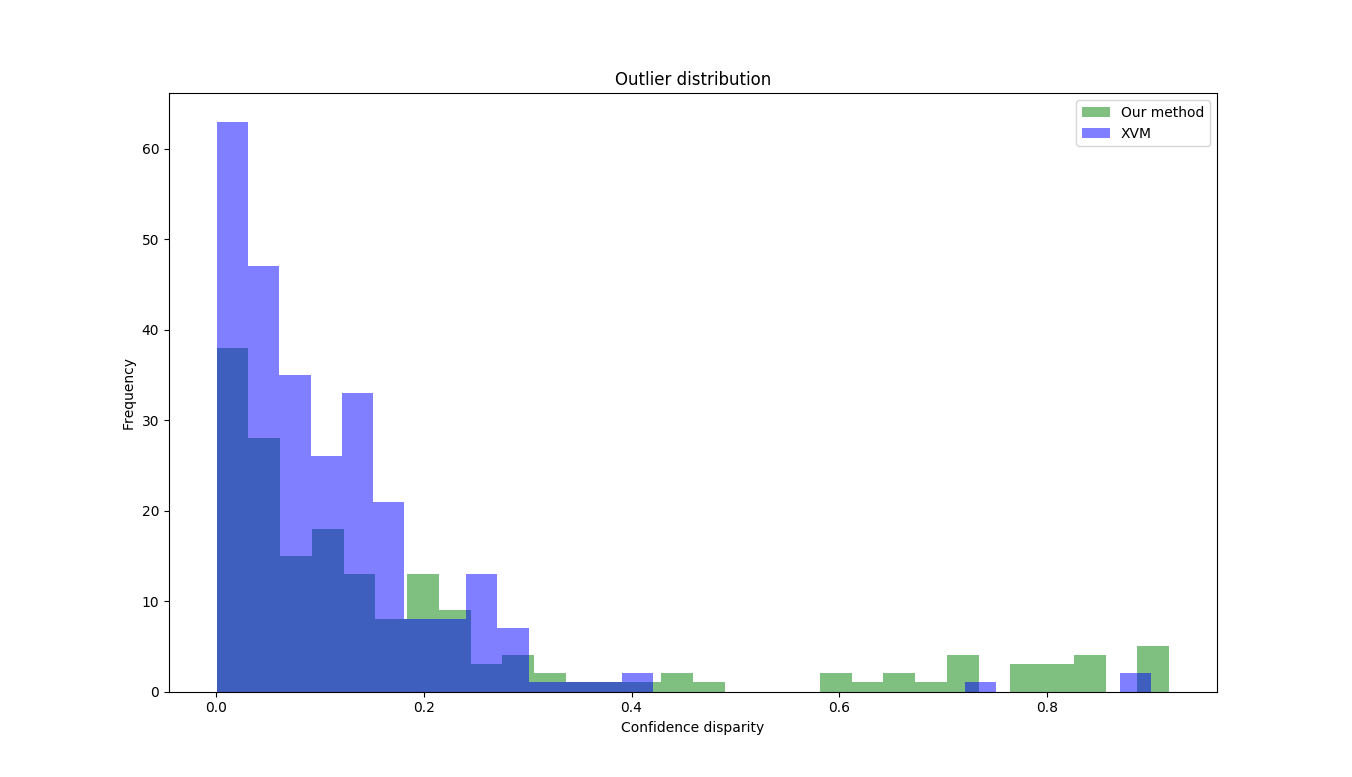
\includegraphics[width=500px]{outliers.png}
  \label{fig:outliers}
\end{figure}

\section{Conclusion}

In this work we briefly overviewed the possibility of using machine learning to predict a game outcome. We conclude, that the work has been partially successful, achieving rather high prediction accuracy, but has deficiencies such as frequent missclassifications for games, that are not severely unbalanced and overconfidence in deciding those, that are fairly balanced.

We suppose that part of the reason for these negative traits is an insufficient number of training samples. Given how variable can two teams of 15 players with 500 tanks available get, few thousand game instances might not be enough to fully train all of the important dependencies.

As to why we were not able to achieve higher accuracy, we reason that the nature of the game and player behaviour is to blame. 
Many times completely unpredictable events happen during the game that swiftly turn the tides in the favor of the other team.

We hope to present some hand-picked outliers showing this during the defense part of this project.

In terms of possible improvements, we could try to create a more sofisticated dataset that handles more parameters than the 3 we used.

One useful by-product of our work is the finding that the WN8 metric is not actually all that important. Whenever we tried to incorporate it in our models (be it heuristic or neural network) the prediction accuracy plummeted. The particular tank used by player seems to matter much more, as the global winrate parameter had the most positive influence in our tests.

\end{document}
